\documentclass{article}
\usepackage[utf8]{inputenc}

\usepackage[parfill]{parskip}
\usepackage[a4paper, total={6in, 10in}]{geometry}

\usepackage{amsmath}

\usepackage{graphicx}
\usepackage[center]{caption}
\usepackage{subcaption}

% Path to images
\graphicspath{./Code/src/matlab/figs/}


\usepackage{float}

\title{Team 2: Multi agent maze exploration}
\author{ Mårten Nilsson \texttt{marten3@kth.se}, Patrik Barkman
  \texttt{barkm@kth.se} \\ Axel Demborg \texttt{demborg@kth.se}, Elon Såndberg
  \texttt{elons@kth.se}}
\date{October 2016}

\begin{document}

\maketitle

\section{Abstract}

\section{Introduction}
%Classical planning... perfect information... exploration necessary... multiagent coordination...

Generating maps of certain areas of importance has long been a question of great interest in a
wide range of fields. Historically the explorers of the areas have been humans.
Though using humans for exploring certain areas is intractable. Both due to
limitations of human capabilities and risks associated with the exploration
task. For an example, during search and rescue operations in hostile
environments such as a building on fire one is not inclined to put more human
lives at risk than necessary. With the recent advances in AI and robotics,
another opportunity for these situations arises. The exploration could be
performed by specialized robots. This does not put any unneccessary human lives
at risk and could possibly lead to a more efficient operation.

One of the greatest challenges for automated multi agent exploration is how to
coordinate the agents in the unknown area. Depending on the limitations of the
robots in the terrain, different methods of addressing the problem arises. In
this report the focus is on some of the established algorithms in the field as
well as proposing some modifications. This study seeks to obtain data to provide
new knowledge of how these algorithms perform in a maze like environment where
conventional heuristics not always result in decent performance.

\section{Related work}
A considerable amount of literature has been published on multi agent
coordination motivated by search and rescue operations. Ferranit, Trigoni and
Levene proposed the \textit{Brick\&Mortar} algorithm in which the agents operate
on local information and communicate indirectly with each other by leaving
information tags at visited points \cite{ferranti2007brick}. Their algorithm is
inspired by the \textit{Ants} algorithm proposed by Koenig and Liu \cite{koenig2001terrain} and the
\textit{Multiple depth first search (MDFS)} algorithm which first occured in \cite{tarry1895probleme}. 

Traditionaly, the problem of multi agent exploration have been seen as a
distinct part of serarch and rescue operations. However, Becker, Blatt and
Szczerbicka proposed the flooding algorithm \cite{becker2013multi} in which the
exploration and rescue parts of the operation work in parallell. In their
algorithm the exploration agents act on local information and frequently report
back to a base of operations.

\section{Problem formulation}
A twodimensional maze-like environment is chosen as the setting in which to
evaluate different approaches to the problem of map generation/exploration.
The only obstacles that exist in the environment are walls through which the
agents cannot pass. A number of agents are positioned in the environment and
their task is to explore the maze as effectively as possible.

The environemnt is represented as a two dimensional grid where each cell can
either be empty or a wall. In addition, the agents can leave traces in cells
they pass in order to indicate to other agents that the cell has previously
been visited. The agents are allowed to move to one of the (non-diagonally)
adjacent cells at each time step. 

A number of algorithms have been studied and they use different assumptions of
how much information each agent can access. Some of the algorithms only use
information of the cells nearby each player while others assume unrestrained
communcation between the agents and knowledge of all the discovered cells.

These assumptions and  constraints and on the environment imply many
simplifications of real life scenarios such as search and rescue operations,
but the environemnt should still suffices to obtain a baseline of the
algorithm's efficiency.

The mazes used for testing are generated with Prim's algorithm
\cite{prim1957shortest}. In order to simplify the maze to obtain an environment
which contains something more similar to isolated obstacles, some walls may be
randomly removed.

\begin{figure}[H]
    \centering
    \begin{subfigure}[b]{0.3\textwidth}
        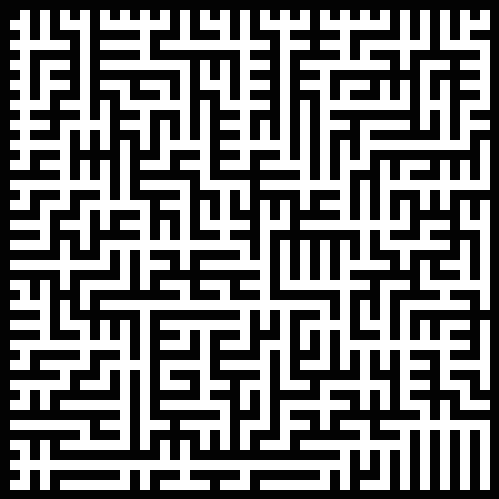
\includegraphics[width=\textwidth]{./maze_easyfy_1.png}
        \caption{Complete maze. No walls removed.}
    \end{subfigure}
    \quad \quad
    \begin{subfigure}[b]{0.3\textwidth}
        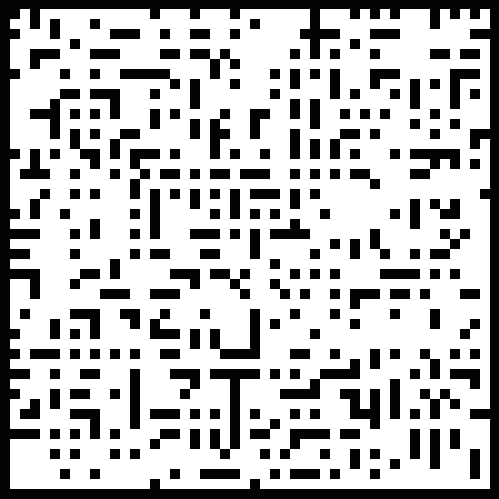
\includegraphics[width=\textwidth]{./maze_easyfy_05.png}
        \caption{Each wall is removed with probability 0.5.}
    \end{subfigure}
    \caption{Mazes generated by Prim's algorithm and simplified by removing
    walls.}
\end{figure}

\section{Method(s)}

\subsection{Ants}
A number of different techniques have been developed to coordinate multiple
agents in exploration tasks. The \textit{Ants} algorithm is a commonly used
technique for this. In the \textit{Ants} algorithm, the agents communicate with
eachother through a pheromone. Each cell contains a certain
pheromone level. When an agent visits a cell, the pheromone level of the cell is
increased. The desicion making process of the agents is designed such that an
agent chooses to move to the neighbouring cell with the lowest pheromone level.

This desicion process is as the name of the algorithm suggests, inspired by
ants. A major advantage of the \textit{Ants} algorithm is that the
agents only operate on local information. Moreover, the desicion making process is
fast and computationally efficient. The algorithm also guarantees that the whole
maze will be explored in finite time. On the other hand the nature of the model
can cause ants to get stuck in local areas of low pheromone levels for quite
some time before the level has risen enough so that the ants can move on towards
unexplored spaces. This may cause an unneccessary high level of revisitations of cells.

\subsection{Multiple Depth First Search (MDFS)}
The problem to discover all the cells in the maze can easily be seen as a search
problem where we want to find all the cells. This is a problem that would
normally be solved with a search algorithm such as \textit{Depth First Search}
and with some minor modifications this algorithm can also be used for multiple
collaborating agents. The algorithm works as follows.

\begin{enumerate}
\item If there are neighboring \textit{unvistited} cells
  \begin{enumerate}
  \item move to one of the \textit{unvistited} cells at random.
  \item mark the cell as \textit{explored} with the agents ID.
  \item mark the cell with the direction of the previous cell, the \textit{parent cell} 
  \end{enumerate}
\item Else if the current cell is marked as explored by the current agent
  \begin{enumerate}
  \item mark the cell as \textit{visited}
  \item move to the \textit{parent cell}
  \end{enumerate}
\item Else if there are \textit{explored} cells around.
  \begin{enumerate}
  \item Move to one of them at random.
  \end{enumerate}
\item Else
  \begin{enumerate}
  \item terminate
  \end{enumerate}
\end{enumerate}

If this procedure is repeated until all agents have terminated it is guaranteed
that the entire environment will be visited and if there is only one agent each
cell will be visited exactly twice, once to mark it as explored and once to
mark it as visited. With multiple agents the guarantee that all cells will be
visited remains but cells might be visited more than once when the agents are
moving along cells explored by other agents. The algorithm also suffers from the
problem that agents can be locked in behind visited cells early in the search
and hence be rendered useless. Like the \textit{Ants} algorithm \textit{MDFS}
only utilizes locally stored information which makes it well suited for
situations when communication between agents is hard and computational resources
are scarce.
\subsection{Deep Ants}
In the current problem formulation, the agents are assumed to be able to
communicate directly with eachother. Therefore algorithms which are created to
operate only on local information may be modified for increased performance. The
\textit{Deep Ants} algorithm is a mofication of the \textit{Ants} algorithm
where this knowledge is used.

The \textit{Deep Ants} algorithm is in the same manner as the \textit{Ants}
algorithm a decentralized planning algorithm where the agents plan their actions
individually and independently of eachother, with respect to the current state
of the area. There is two key differences
between the \textit{Deep Ants} algorithm and the \textit{Ants} algorithm. The
first difference is that when an agent visits a cell in the \textit{Deep Ants}
algorithm, not only is the pheromone level of the cell increased by a level $l_1$ but also the
pheromone level of the neighbouring cells are increased by a level $l_2$ so that
$l_2 * n = l_1$. Here $n$ is a parameter which controls the ratio of the
pheormone levels. 

The other key difference between the \textit{Deep Ants} and the \textit{Ants}
algorithm is the desicion making process. In the regular \textit{Ants} algorithm
the goal is to minimize the encountered pheromone level in the next step for the
agent. In the \textit{Deep Ants} algorithm the goal is to move to the cell
$\mathbf{x}$ that minimizes

$$ p_d(\mathbf{x}) = p_1(\mathbf{x}) + \begin{cases} \text{min}_i
  \left(p_{d-1}(\mathbf{x_i}) \right)  & \text{if } d > 1 \\
  l(\mathbf{x}) & \text{if } d = 1 \end{cases}$$

where $l(\mathbf{x})$ is the pheromone level at cell $\mathbf{x}$ and
$\mathbf{x_i}$ is the i:th cell that is adjecant to cell $\mathbf{x}$. The index
$d$ is the search depth and is a parameter in the model. This means that the
agents in the \textit{Deep Ants} algorithm tries to minimize the total amount of
encountered pheromone in the next $d$ steps.  

It is important to keep in mind that it is impossible for the agents to know
what moves can be performed in the unexplored area. In this algorithms the
Agents are naive and assumes every move is possible outside of the explored area.

The benefit of the \textit{Deep Ants} approach compared to the \textit{Ants}
algorithm is that the agents can chose to move to areas of higher pheromone
levels in case there is a low feromone area on the other side of it. Therefore
it should be less likely that the agents be trapped in a smaller area a longer
period of time. The cost of this is that the algorithm is more computationally
demanding and requires a collective knowledge base.

\subsection{Decentralized Search with Global Information}

\subsection{Centralized Search with Global Information}
In addition to the methods based on decentralized planning, attempts have been
made to device an algorithm with centralized planning using global information.
Such an algorithm could be realizable in environments where all agents are able
to communicate with a centralized system. Theoretically, this approach should
be the most effective, but also the most computationally demanding. This is
mainly due to the dimension of the search space grows exponentially with the
number of agents.

The method is based on the $A^*$ search algorithm. It is an informed search
where states are prioritized according to the cost function
%
$$f(x) = g(x) + h(x)$$
%
where $g(x)$ is the cost of traversing from the start to the state $x$ and
$h(x)$ is an heuristic that estimates the cost from $x$ to the goal. In this
case the start state consists of any possible placement of the agents in the
enviroment and in genernal the environment has only partly been explored by the
agents. The goal state is defined such that all the agents should be positioned
on a border to an undiscovered area of the environment. Since the agents will
have to travel different distance to reach such a border, as soon as one agent 
has found its way to the border its position is no longer varied during the 
remaining search.

The function $g(x)$ is defined as
%
$$g(x) = a * \begin{Bmatrix} \text{number of steps} \\ \text{from start to $x$}
\end{Bmatrix} + b * \begin{Bmatrix} \text{explored area at start} \\ - \\ \text{
explored area at $x$} \end{Bmatrix}$$
%
Since the goal is defined as above, the second term effectivley only matters
when the search is one step from the goal. This choice of cost function should
inclince the agents to prioritize goals that are close and approach that area in
such a way as to discover as large area as possible.

The heuristic $h(x)$ is defined as 
%
$$h(x) = c * \text{\{distance to nearest undiscovered area\} }$$
%
Since this underestimates the actual cost it is an admissible heuristic 
\cite{russell2003artificial}. The heuristic is crucial in order to guide the 
search in the right direction and consequently avoiding extensive computations.
This heuristic is in practice an estimate of the first term in $g(x)$ ---
unknown areas that are closer to the agent is prioritized.

In the case study explained below the coefficients $a = 10$, $b = 1$ and $c =
1$ were used.

\subsection{Centralized Search with Global Information with individual search}
An attempt to make a less computationally demanding centralized search with global information was made.
The method searched the known map for each agent ignoring all other agents in order to cut down the branching factor of the search. Each agent searches for it's closest unexplored cell, when this cell is found it is marked with the number distance in steps to the agent and future agents will ignore this cell in their searches if they cannot walk to using fewer steps than what it has been marked for. If the agents fails to find a cell because all cells are marked it unmarks all the cells and searches again. This is done to prevent agents from not moving since staying in unexplored territory will be worse than moving towards an unexplored cell that another agent is heading towards.

A version of the algorithm was tried where the agents searched for a new cell to walk towards if another agent was closer to the cell it was trying to walk towards. This should theoretically make the algorithm better but the computational power required increases quite a lot and the efficiency gained is marginal since all the agents will move towards the unexplored horizon either way and a small difference in exact goal does not make much of a difference. There are however many other ways to speed up the performance of this algorithm, such as keeping track of the number of unexplored reachable cells in order to know when to clear the marks off the cells without having to search through all the cells first. Another way to optimize this algorithm would be to save the whole path towards the target for each agent so that if no new information has been gained from one game state to the next all agents does not have to do a new search since their targets will be unchanged. All of this will only increase the time performance of the algorithm and not the number of steps to explore the space, because of this and time constraints these optimizations were not implemented.


\section{Case study}
A case-study approach was adopted to obtain further in-depth information of the
performance of the previously mentioned algorithms within the constraints of
the current problem formulation. All algorithms were tested with three agents
exploring a $50 \times 50$ prims maze reduced by $0 \%, 50 \% $ and $100\%$, where the
reduction was performed by randomly replacing wall cells with free space cells.
The performance of the algorithms was evaluated by measuring both exploration
percentage as a function of number of iterations and as a function of time.


For the algorithms with the ability to scale to higher number of agents for this
maze size, the same test was performed for $10$ and $100$ agents for maze sizes
$50 \times 50$ and $100 \times 100$. 


\section{Performance measures}
To be removed...
\begin{itemize}
\item Exploration percentage vs number of iterations
\item Exploration time vs number of agents
\item Time per iteration vs number of iterations
\end{itemize}

\section{Results}

\begin{figure}[H]
    \centering
    \begin{subfigure}[b]{0.3\textwidth}
        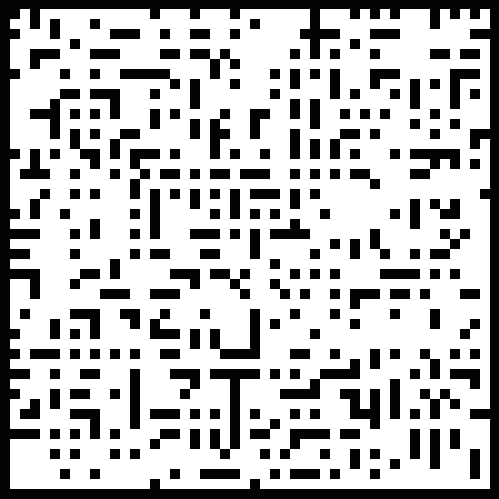
\includegraphics[width=\textwidth]{./maze_easyfy_05.png}
        \caption{Complete maze. No walls removed.}
    \end{subfigure}
    \quad \quad
    \begin{subfigure}[b]{0.3\textwidth}
        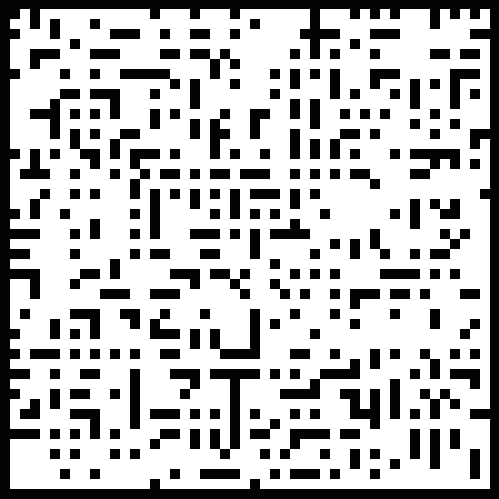
\includegraphics[width=\textwidth]{./maze_easyfy_05.png}
        \caption{Each wall is removed with probability 0.5.}
    \end{subfigure}
    \caption{Mazes generated by Prim's algorithm and simplified by removing
    walls.}
\end{figure}



\section{Discussion}

\begin{itemize}
    \item Why not test Brick\&Mortar? -MDFS not optimal in our setting etc...
    \item Heuristic of Global Player should be better
    \item Popssible optimizations of algorithms and consequences of this
\end{itemize}

\section{Conclusions}


\bibliographystyle{unsrt}
\bibliography{references}


\end{document}
